%\VignetteIndexEntry{introduction}
\documentclass{article}

%%% latex packages
\usepackage{hyperref}
\usepackage[utf8]{inputenc}
\usepackage[usenames,dvipsnames]{xcolor}

\usepackage{lipsum} % for dummy text only

%% change margins to 1" all the way around
\oddsidemargin 0.0in
\evensidemargin 0.0in
\textwidth 6.5in
\headheight 0.0in 
\topmargin 0.0in
\textheight 9.0in

%%% document info
\title{Introduction to \texttt{SpaDES}}

\author{
  Alex M. Chubaty\\
	\small{Natural Resources Canada, Pacific Forestry Centre}\\
	\small{email: \href{mailto:achubaty@nrcan.gc.ca}{achubaty@nrcan.gc.ca}}
	\and
	Eliot McIntire\\
	\small{Natural Resources Canada, Pacific Forestry Centre}\\
	\small{email: \href{mailto:emcintir@nrcan.gc.ca}{emcintir@nrcan.gc.ca}}
}

\usepackage{Sweave}
\begin{document}
\Sconcordance{concordance:introduction.tex:introduction.Rnw:%
1 31 1 1 0 14 1 1 3 2 0 1 1 1 10 8 0 1 2 7 0 1 5 14 1 1 2 1 0 4 1 1 2 4 %
0 1 2 22 1 1 2 1 0 1 4 2 0 1 2 1 0 3 1 1 5 3 0 1 1 1 2 11 0 1 1 15 0 1 %
7 5 0 1 2 5 0 1 2 7 1}

 % displays code as entered (no arranging lines)

\maketitle

\tableofcontents

\newpage

\section{Spatial Discrete Event Simulation (SpaDES)}

\paragraph{Requirements}
This packages makes heavy use of the \texttt{raster} and \texttt{sp} packages, so familiarity with these packages and their classes and methods is recommended.

\begin{Schunk}
\begin{Sinput}
> ## for now only while testing, etc.
> OS <- tolower(Sys.info()["sysname"])
> hostname <- gsub(Sys.info()["nodename"],pattern="W-VIC-",replace="")
> if (OS=="windows") {
+     if(pmatch("A105200", hostname, nomatch=FALSE)) {
+         path <- "c:/Eliot/GitHub"
+     } else {
+         path <- "~/GitHub"
+     }
+ } else {
+     path <- "~/Documents/GitHub"
+ }
> #devtools::dev_mode(TRUE)
> devtools::load_all(file.path(path, "SpaDES")) # for development/testing
> 
> ## 
> #library(SpaDES)
\end{Sinput}
\end{Schunk}


\newpage

\section{SpaDES modules}

\lipsum

\newpage

\section{Working with maps}

\paragraph{A raster map}
Sample map of habitat quality.

\begin{Schunk}
\begin{Sinput}
> nx = 1e3
> ny = 1e3
> habitat = raster(nrows=ny, ncols=nx, xmn=-nx/2, xmx=nx/2, ymn =-ny/2, ymx=ny/2)
> habitat = round(GaussMap(habitat, speedup=10), 1)
> names(habitat) = "habitatQuality"
> simPlot(habitat)
\end{Sinput}
\end{Schunk}
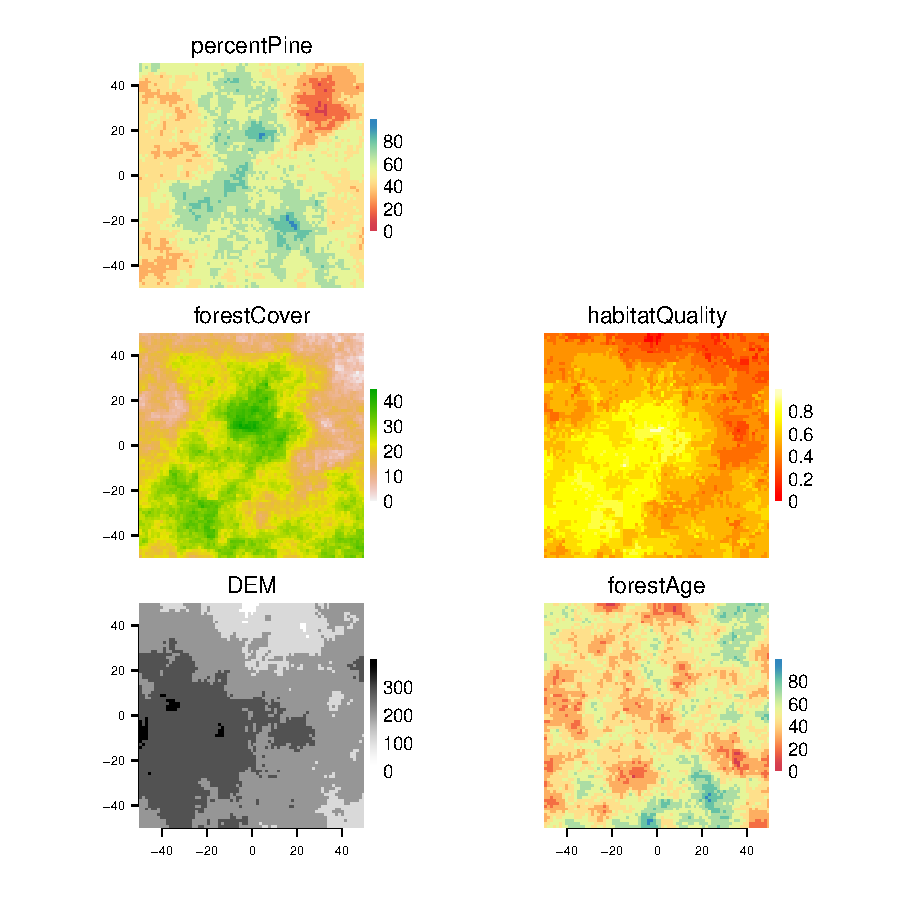
\includegraphics{introduction-habitat-map}

\newpage

\section{Simulating ``agents''}

\paragraph{}

\subsection{Spatial agents}

\subsubsection{Point agents}

\paragraph{}
Agents represented by a single set of coordinates indicating their current position.

\paragraph{}
Use a \texttt{SpatialPointsDataFrame} with additional columns as needed.

\paragraph{Non-mobile point agents}
e.g., plants

\paragraph{Mobile point agents}
e.g., animals use a \texttt{SpatialPointsDataFrame}, with additonal columns for agents' previous \texttt{n} positions, and any other columns such as age, sex, group membership, etc.

\begin{Schunk}
\begin{Sinput}
> N <- 10 # number of agents
> # caribou data vectors
> IDs <- c("Alice", "Bob", "Clark", "Daisy", "Eric",
+          "Franz", "Gabby", "Hayley", "Igor", "Jane")
> sex <- c("female", "male", "male", "female", "male",
+          "male", "female", "female", "male", "female")
> age <- round(rnorm(N, mean=8, sd=3))
> prevX <- rnorm(N, mean=0, sd=100) # previous X location
> prevY <- rnorm(N, mean=0, sd=100) # previous Y location
> # create the caribou agent object
> caribou <- SpatialPointsDataFrame(coords=cbind(x=rnorm(N, mean=0, sd=100),
+                                                y=rnorm(N, mean=0, sd=100)),
+                                   data=data.frame(prevX, prevY, sex, age))
> row.names(caribou) <- IDs # alternatively, add IDs as column in data.frame above
> head(caribou)
\end{Sinput}
\begin{Soutput}
          prevX     prevY    sex age
Alice  54.99758 130.16838 female   5
Bob    56.14550 -95.23294   male   6
Clark  43.69673  15.60575   male   6
Daisy  73.21684 -53.28818 female   4
Eric  -98.50261 -40.84025   male   9
Franz -91.65131 -86.06384   male   8
\end{Soutput}
\begin{Sinput}
> coordinates(caribou)
\end{Sinput}
\begin{Soutput}
                x          y
Alice   166.54789  -88.76219
Bob      76.09910  -33.91571
Clark  -179.22315  -46.17070
Daisy    18.61346   11.46486
Eric    141.21491   38.41175
Franz   203.02519  -41.98872
Gabby   144.57089   25.48473
Hayley   54.52718 -139.59689
Igor     68.74024  -65.12978
Jane    -13.99476 -151.89578
\end{Soutput}
\begin{Sinput}
> ## conventional plotting method
> #plot(habitat)
> #plot(caribou, add=TRUE)
> 
> # improved plotting using simPlot
> simPlot(habitat)
> simPlot(caribou, ext=extent(habitat), on.which.to.plot=1, add=TRUE, pch=19,
+         gp=gpar(cex=0.1), delete.previous=FALSE)
\end{Sinput}
\end{Schunk}
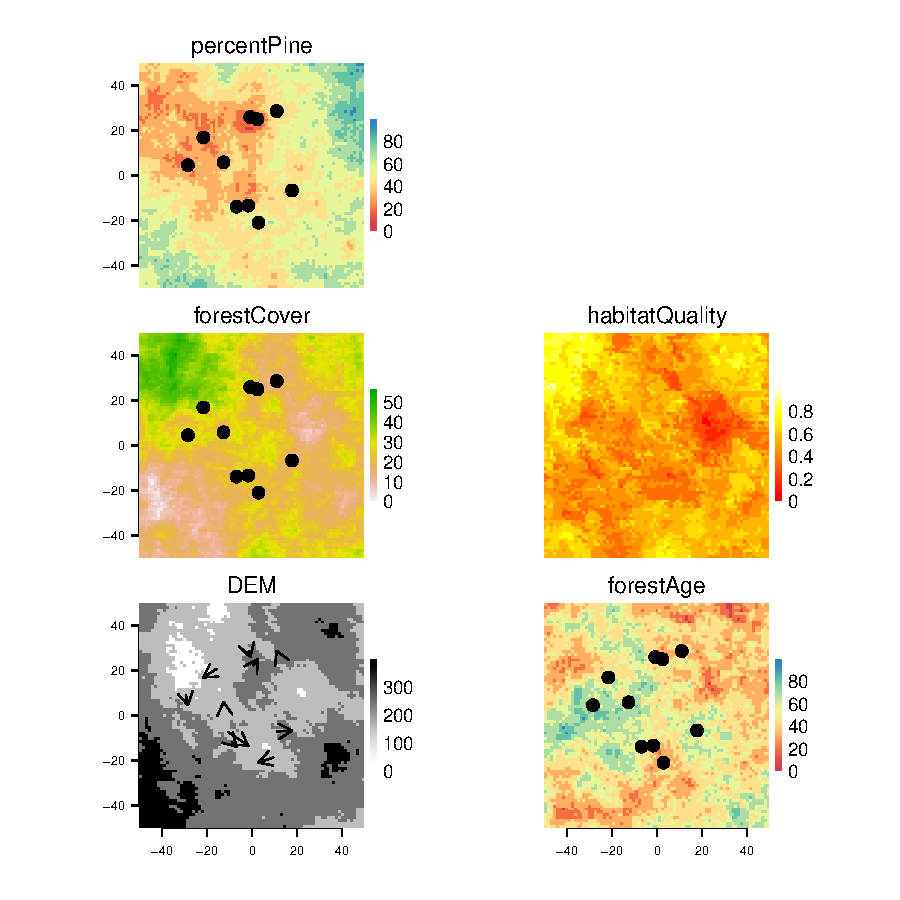
\includegraphics{introduction-mobile-point-agent}

\newpage

\section{A simple individual based model (IBM)}

\lipsum

\end{document}
